\begin{appendices}

\chapter{Appendices}
\label{ch:appendices}

\section{Appendix A - Deployment Roles \& Users}
\label{appendix:roles_users}

Mind Map representing the identified user roles of the Department of Computing Science in red to the left and the identified users in blue to the right.

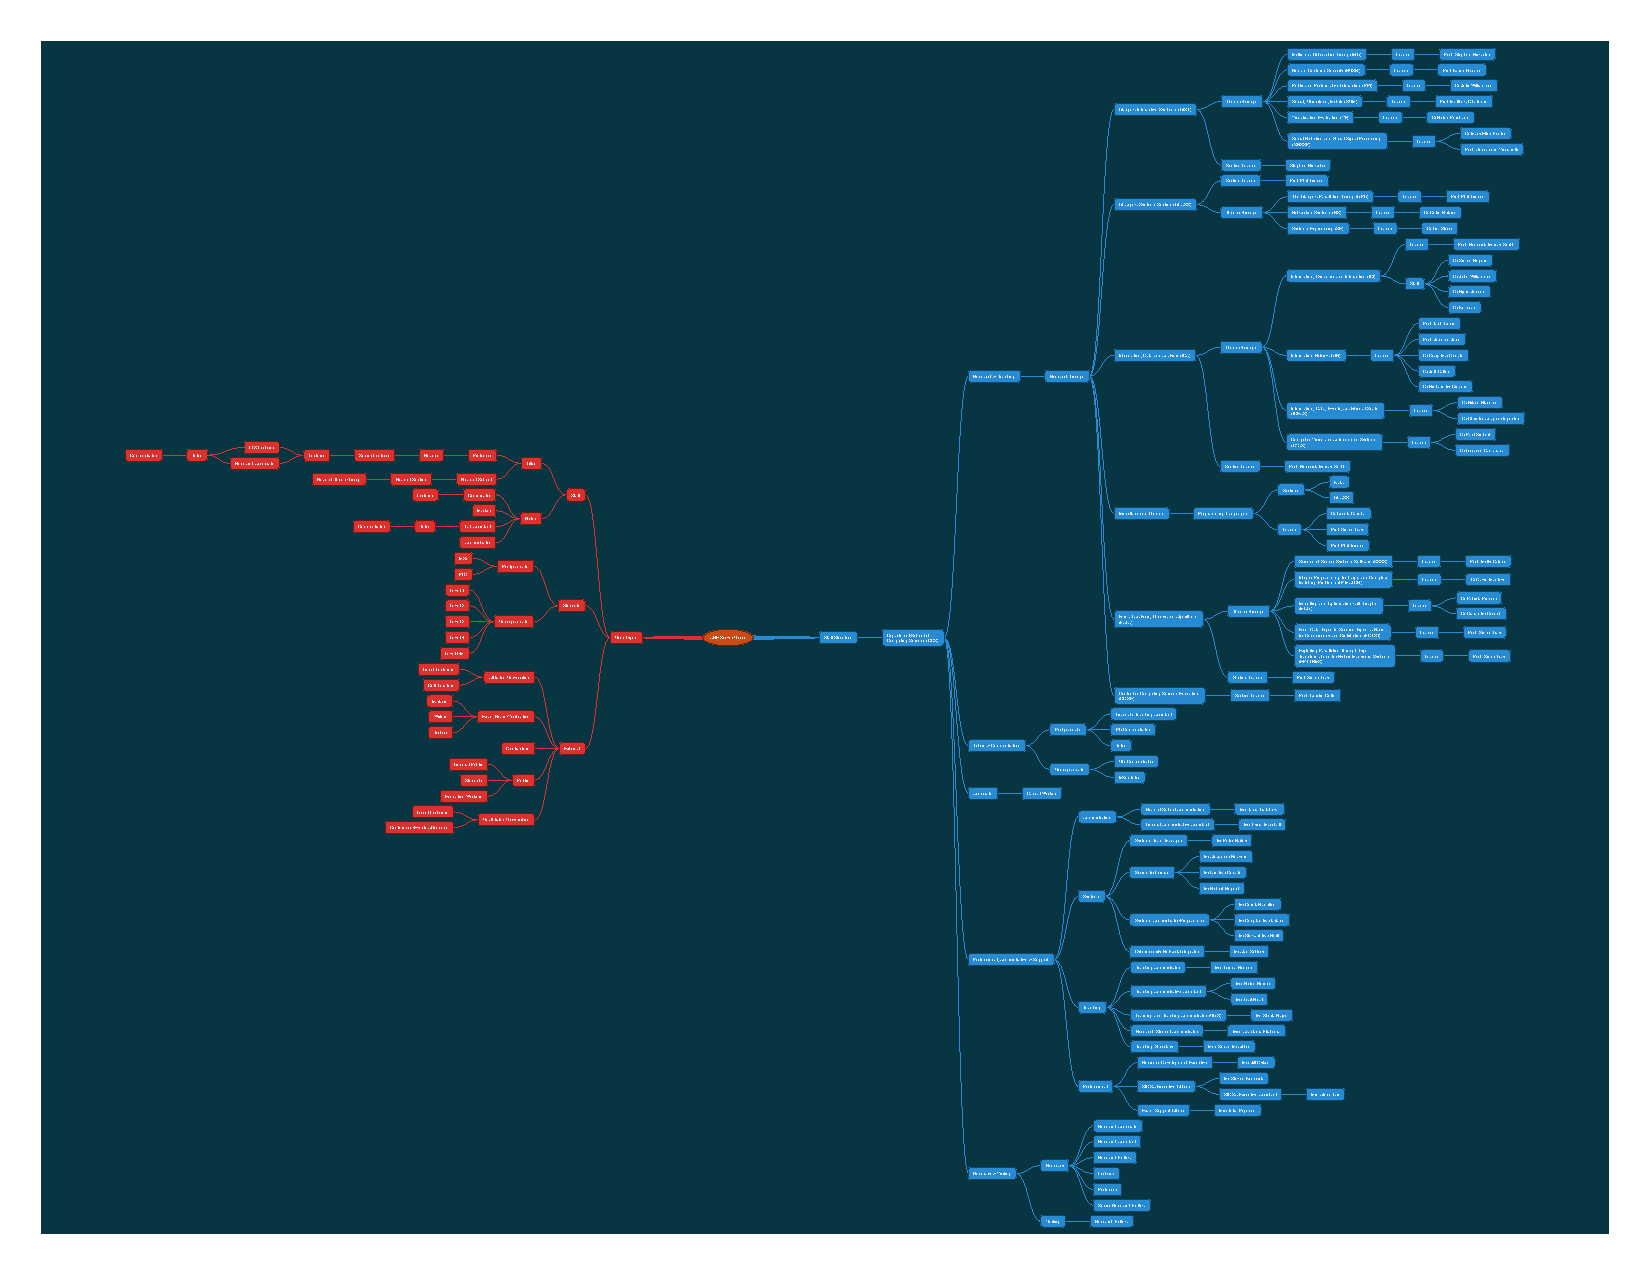
\includegraphics[width=\linewidth]{appendices/mind_maps/ABE_Users_slides_Oct26.pdf}

\section{Appendix B - Enrolment Diagram for Staff User}
\label{appendix:enrolment_diagram}

\begin{figure}
    \centering
    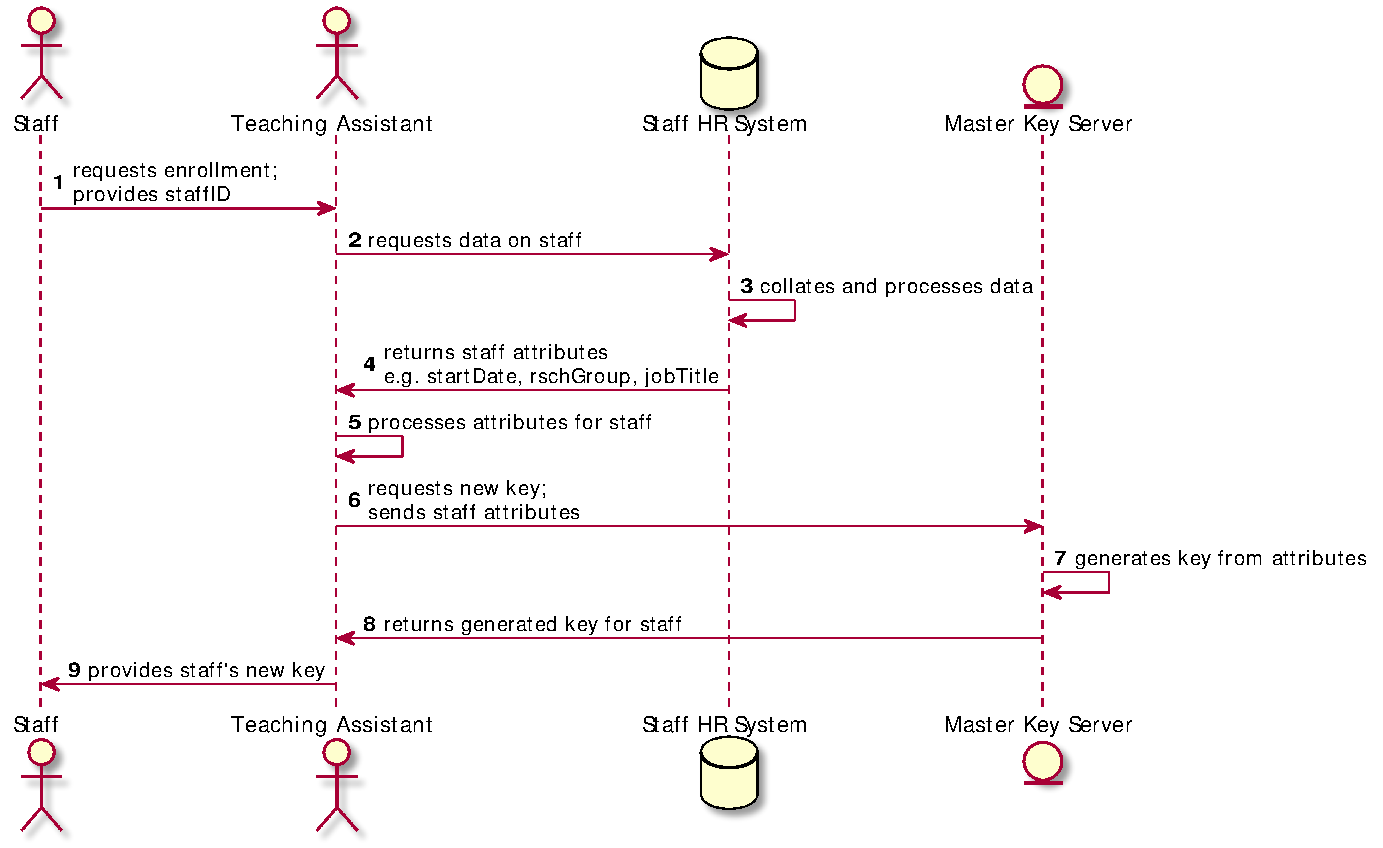
\includegraphics[width=\linewidth,keepaspectratio]{appendices/diagrams/flow_of_info/enrollment_sta_sequence.pdf}

    \caption{A sequence diagram demonstrating the enrolment process for a staff member. The staff member can be seen requesting a user key \#1 (and providing their staff username) from the \acrshort{dcs} Teaching Assistant, whom verifies the staff members's identity and then retrieves their details \#2 from the HR/Payroll system. The Teaching Assistant then processes the returned attributes \#5 for the Master Key Server, and then requests a new key \#6 by providing the student's attributes. The Master Key Server can be seen processing \#7 and then returning the newly generated key \#8 to the Teaching Assistant, whom finally provides the key to the staff member.}

\end{figure}

\section{Appendix C - System Architecture Diagram}
\label{appendix:architecture_diagram}

\begin{figure}
    \centering
    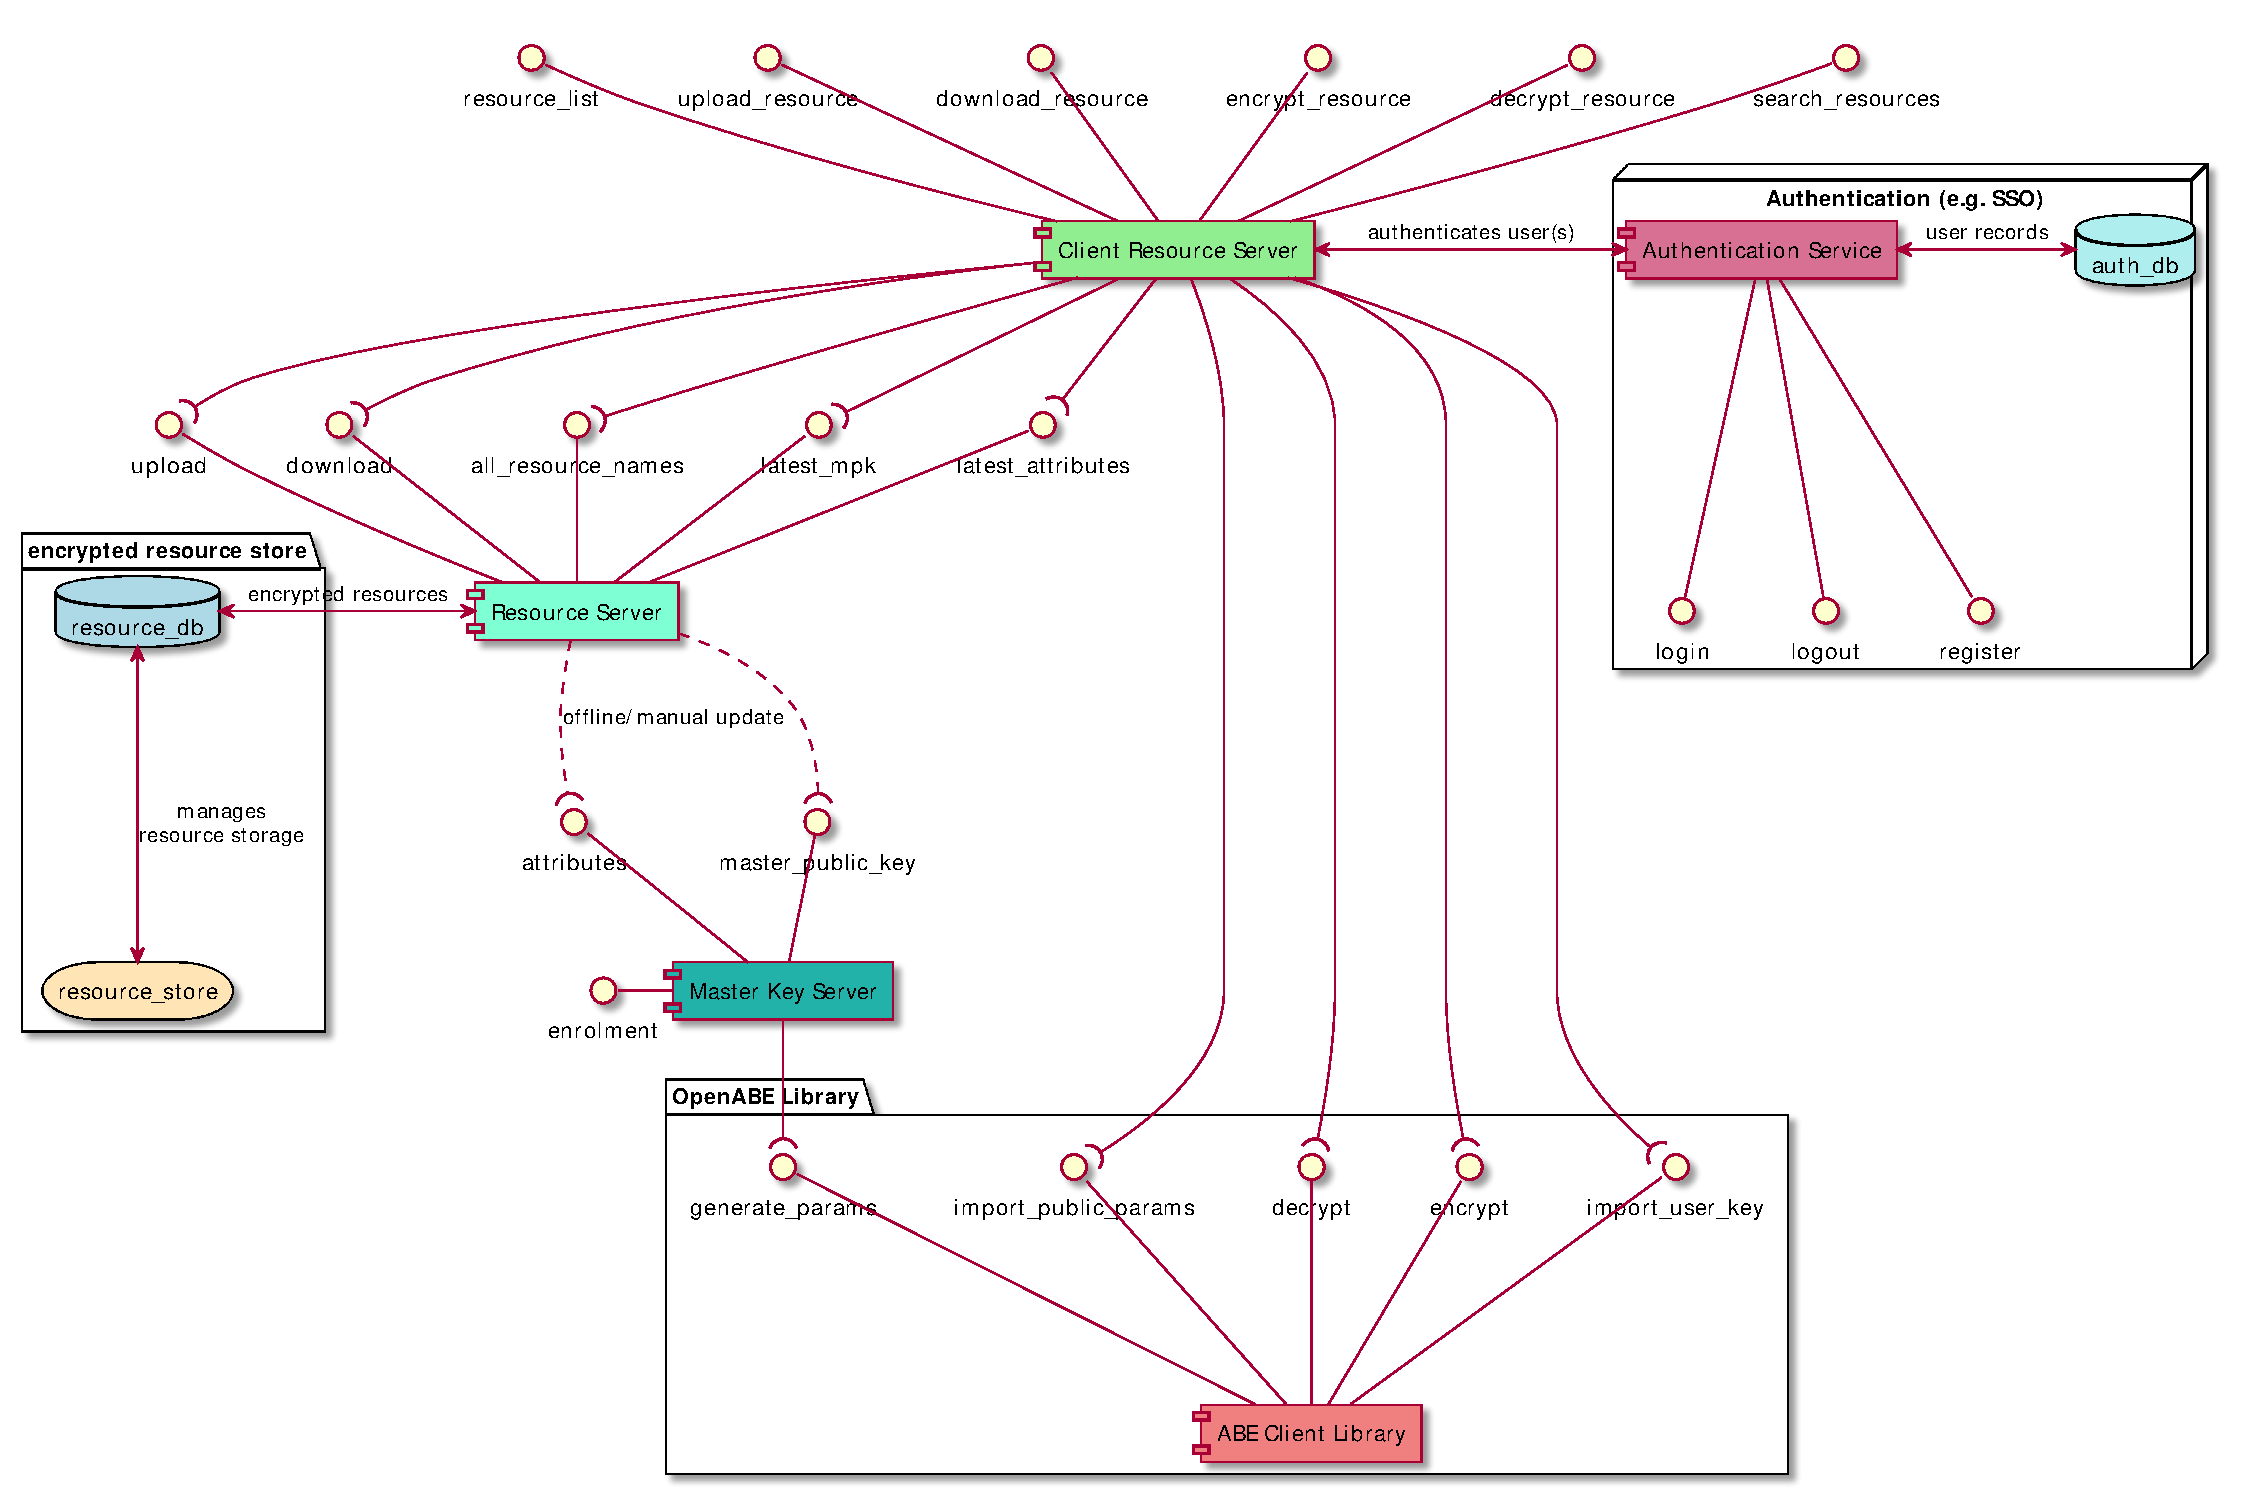
\includegraphics[width=\linewidth,keepaspectratio]{appendices/diagrams/infrastructure/system_architecture.pdf}

    \caption{
      A full architecture diagram describing the system architecture of the \theResServer system.
      The \acrfull{mks} is shown in an offline state with access to a local copy of the \OpenABE library for provisioning the system \& generating user keys. The \acrfull{prs} is shown receiving offline updates from the \acrshort{mks}, managing a local database with resource metadata \& the associated resource storage and providing search, config and upload \& download interfaces for clients. The \acrfull{crs} is shown with local access to an \OpenABE library for encryption \& decryption and access to an abstract Authentication Service (such as the university's SSO system). The \acrshort{crs} also implements the search, config and upload \& download interfaces provided by the \acrshort{prs} and provides its own upload \& download, encrypt \& decrypt and resource search interfaces for the user.
    }

\end{figure}

\section{Appendix D - Case Study \#0 Policy}
\label{appendix:case_study_0_policy}

For this study the following details have been assumed:
\begin{itemize}
  \item
    the solutions were encrypted and then uploaded by the Admin staff member
  \item
    the staff member is Teresa Bonner with username `tbonner'
\end{itemize}
\vskip 0.5em
With the details extracted, we can determine the attributes for the policy, where we define \textbf{\textit{Subject} s} and \textbf{\textit{Environment} e} as:
\begin{itemize}
  \item[]
    \textbf{s} $\Rightarrow$ role, accountActiveUntil, username
  \item[]
    \textbf{e} $\Rightarrow$ currentDate
\end{itemize}

Applying the identified attributes for Case Study \#0 (\Cref{subsec:analysis_case_studies_0}) provides the policy in \cref{fig:case_study_policy_0} which would have been embedded in the encrypted lecture slides by the staff member before upload. The encrypted past paper can then remain stored on the server but only accessible to staff members and students.

\begin{figure}[ht]
  \centering
\begin{align*}
  \text{Policy(\textbf{s},\textbf{e})}
  &
    \leftarrow
    \text{username(\textbf{s})} \equiv \text{`tbonner'}
  \\
  &
    \phantom{::}\vee
    \text{role(\textbf{s})} \equiv \text{`Staff'} \mid \text{`Student'}
  \\
  &
    \phantom{::}\wedge
    \text{accountActiveUntil(\textbf{s})} \geq \text{currentDate(\textbf{e})}
\end{align*}
  \caption{
    \label{fig:case_study_policy_0}
    Case Study \#0 policy dictating access to a past exam paper.
    Successful decryption would be possible for the author of the slides (with username `tbonner') \textbf{or} any member of staff \textbf{or} any student. In all cases an active account is also required.
  }
\end{figure}


\section{Appendix E - Case Study \#2 Policy}
\label{appendix:case_study_2_policy}

For the sake of the scenario, the 1P Programming course was selected with Course Code 1001 as it offers the added complexity of tutors \& demonstrators, but it should be remembered that any course with labs could have been chosen.
\vskip 0.5em
For this study the following details have been assumed:
\begin{itemize}
  \item
    the lab solutions have been uploaded in advance of the actual lab date
  \item
    the lab date is scheduled for 04/12/19
  \item
    the solutions were encrypted and then uploaded by the Lecturer
  \item
    the Lecturer for 1001 is John Williamson with username `jwilliamson'
  \item
    Course 1001 is a Level 1 course
  \item
    Course 1001 has a sister course, 1017
  \item
    the 1P course labs are assisted by tutors \& demonstrators from Level 4+
\end{itemize}

\begin{figure}[ht]
  \centering
\begin{align*}
  \text{Policy($sub$, $env$, $res$)}
  &
    \leftarrow
    \text{username($sub$)} \equiv \text{`jwilliamson'}
  \\
  &
    \phantom{::}\vee
    \text{( role($sub$)} \equiv \text{`Staff'}
  \\
  &
    \phantom{::::::::}\wedge
    \text{jobField($sub$)} \equiv \text{`Research \& Teaching' )}
  \\
  &
    \phantom{::}\vee
    \text{( role($sub$)} \equiv \text{`Student'}
  \\
  &
    \phantom{::::::::}\wedge
    \text{studentLevel($sub$)} \equiv \text{1}
  \\
  &
    \phantom{::::::::}\wedge
    \text{enrolledCourses($sub$)} \equiv \text{[1001, 1017]}
  \\
  &
    \phantom{::::::::}\wedge
    \text{currentDate($env$)} \geq \text{7 December 2019 )}
  \\
  &
    \phantom{::}\vee
    \text{( role($sub$)} \equiv \text{`Student'}
  \\
  &
    \phantom{::::::::}\wedge
    \text{studentLevel($sub$)} \geq \text{4}
  \\
  &
    \phantom{::::::::}\wedge
    \text{studentRole($sub$)} \equiv \text{`Demonstrator UG'} \mid \text{`Demonstrator PG'} \mid \text{`Tutor'}
  \\
  &
    \phantom{::::::::}\wedge
    \text{demonstratorCourses($sub$)} \equiv \text{[1001, 1017]}
  \\
  &
    \phantom{::::::::}\wedge
    \text{startDate($env$)} \leq \text{currentDate($env$)}
  \\
  &
    \phantom{::::::::}\wedge
    \text{endDate($env$)} \geq \text{currentDate($env$) )}
  \\
  &
    \phantom{::}\wedge
    \text{accountActiveUntil($sub$)} \geq \text{currentDate($env$)}
\end{align*}
  \caption{
    \label{fig:case_study_policy_2}
    Case Study \#2 policy dictating access to a set of course `1001' lab solutions.
  }
\end{figure}
Applying the identified attributes for Case Study \#2 provides the policy in \Cref{fig:case_study_policy_2} which would have been embedded in the encrypted lab solution by the Lecturer before upload. The encrypted lab solution can then remain stored on the server but will only accessible to the author of the solutions (with username `jwilliamson') \textbf{or} a member of staff in the `Research \& Teaching' field \textbf{or} a Level 2 student enrolled in the `1001' \& `1017' courses if it is 3 days after the lab date of 04/12/19 \textbf{or} a Level 4+ student employed as a demonstrator or tutor that has been assigned to the `1001' \& `1017' course and it is within their dates of employment. In all cases an active account is also required.


\section{Appendix F - Case Study \#4 Policy}
\label{appendix:case_study_4_policy}

In this case, the student has encrypted and uploaded their dissertation to the \theResServer system with access to be granted for their supervisor, the assigned reader and additionally, the Project Coordinator.
\vskip 0.5em
For this study the following details have been assumed:
\begin{itemize}
  \item
    the student has the ID and username `2123456z'
  \item
    their supervisor is Quintin Cutts with username `qcutts'
  \item
    their assigned reader is Paul Siebert with username `psiebert'
  \item
    the Project Coordinator is John Williamson with username `jwilliamson'
\end{itemize}
\vskip 0.5em
Applying the identified attributes for Case Study \#4 provides the policy in \Cref{fig:case_study_policy_4} which would have been embedded in the encrypted dissertation by the student before upload. The encrypted dissertation can then remain stored on the server but only accessible to the student and required staff members.

\begin{figure}[ht]
  \centering
\begin{align*}
  \text{Policy($sub$, $env$, $res$)}
  &
    \leftarrow
    \text{( role($sub$)} \equiv \text{`Student'}
  \\
  &
    \phantom{::::::}\wedge
    \text{username($sub$)} \equiv \text{`2123456z' )}
  \\
  &
    \phantom{::}\vee
    \text{( role($sub$)} \equiv \text{`Staff'}
  \\
  &
    \phantom{::::::}\wedge
    \text{username($sub$)} \equiv \text{`qcutts'} \mid \text{`psiebert'} \mid \text{`jwilliamson' )}
  \\
  &
    \phantom{::}\wedge
    \text{accountActiveUntil($sub$)} \geq \text{currentDate($env$)}
\end{align*}
  \caption{
    \label{fig:case_study_policy_4}
    Case Study \#4 policy dictating access to a completed dissertation.
    Successful decryption would be possible for the author of the dissertation (with username `2123456z') \textbf{or} for the three identified staff members (with usernames `qcutts', `psiebert', `jwilliamson'). In all cases an active account is also required.
  }
\end{figure}


\section{Electronic Appendices}
\label{appendix:electronic_appendices}

We make note of the Risk Assessment Excel document. Too large to submit within the dissertation, it is included in the submitted code file under: \texttt{l4-project-research/reports/RiskAssessment.xlsx}.

\end{appendices}
